\documentclass[twoside]{article}
\usepackage{amsgen,amsmath,amstext,amsbsy,amsopn,amssymb,}
\usepackage{graphicx}
\usepackage{epsfig}

\setlength{\oddsidemargin}{0.1 in} \setlength{\evensidemargin}{-0.1
in} \setlength{\topmargin}{-0.6 in} \setlength{\textwidth}{6.5 in}
\setlength{\textheight}{10.5 in} \setlength{\headsep}{0.1 in}
\setlength{\parindent}{0 in} \setlength{\parskip}{0.1 in}

\newcommand{\homework}[2]{
   \pagestyle{myheadings}
   \thispagestyle{plain}
   \newpage
   \setcounter{page}{1}
   \noindent
   \begin{center}
   \framebox{
      \vbox{\vspace{2mm}
       \hbox to 6.28in { {\bf Math 4720:~Statistical Methods \hfill} }
       \vspace{6mm}
       \hbox to 6.28in { {\Large \hfill #1 (#2)  \hfill} }
       \vspace{6mm}
      \vspace{2mm}}
   }
   \end{center}
   \markboth{#1}{#1}
   \vspace*{4mm}
}

\newcommand{\bbF}{\mathbb{F}}
\newcommand{\bbX}{\mathbb{X}}
\newcommand{\bI}{\mathbf{I}}
\newcommand{\bX}{\mathbf{X}}
\newcommand{\bY}{\mathbf{Y}}
\newcommand{\bepsilon}{\boldsymbol{\epsilon}}
\newcommand{\balpha}{\boldsymbol{\alpha}}
\newcommand{\bbeta}{\boldsymbol{\beta}}
\newcommand{\0}{\mathbf{0}}

\begin{document}

\homework{$7^{th}$ Week Summary}{2/27/25}
\vspace{-0.4 in}
\begin{itemize}
\item In practice, we don't know $\sigma$, so we substitute $s$ for $\sigma$. The resulting statistic does not have a normal distribution.
\item Draw a random sample of size $n$ from a normal distribution with mean $\mu$ and standard deviation $\sigma$. The \textbf{one-sample t statistic}: $t=\dfrac{\bar{x}-\mu}{s/\sqrt{n}}$ has the \textbf{t distribution} with $n-1$ degrees of freedom.
\subitem The p\_value for a test of $H_0: \mu = \mu_0$ against
\subsubitem $H_a: \mu > \mu_0$ is p-value $ = P(T\geq t)$
\subsubitem $H_a: \mu < \mu_0$ is p-value $ = P(T\leq t)$
\subsubitem $H_a: \mu \neq \mu_0$ is p-value $ = 2P(|T|\geq|t|)$
\subitem These p-values are exact if the population distribution is Normal; they are approximately correct for large $n$ in other cases.
\item the $t$ distribution with $n-1$ degrees of freedom approaches the standard normal distribution $N(0,1)$ as $n$ increases.
\item Confidence interval for $\mu$ is $\bar{x} \pm t_{\alpha/2}\dfrac{s}{\sqrt{n}}$ with $df=n-1$, if
\subitem data is coming from normal population having unknown mean $\mu$ and unknown $\sigma$, or
\subitem large random sample from a non-normal population having unknown mean $\mu$ and unknown $\sigma$.

\end{itemize}
\vspace{-.25in}\hrulefill\vspace{-.15in}

\begin{itemize}
\item \textbf{Comparing the means of two populations}\dotfill
\item \textbf{Independent samples }: A so-called two-sample problem can arise from a \textit{randomized comparative experiment} that randomly divides subjects into two groups and exposes each group to a different treatment.
\subsubitem To perform inference about $\mu_1 - \mu_2$, the difference between the means of the two populations, we start from $\bar{x}_1 - \bar{x}_2$, the difference between the means of the two samples.
\end{itemize}
\vspace{-.3in}
\begin{figure}[h]
\begin{center}
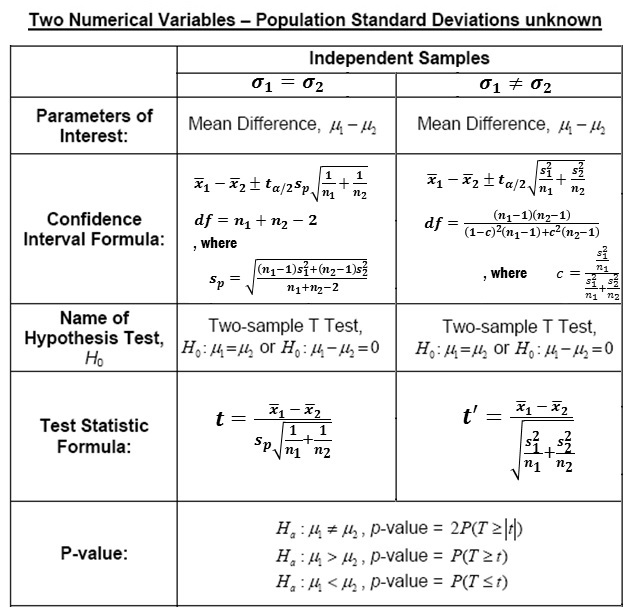
\includegraphics[angle=0, width=11.5 cm] {HT_2.jpg}
\end{center}
\end{figure}

\end{document}


